\documentclass{report}
\usepackage[T1]{fontenc} % Fontes T1
\usepackage[utf8]{inputenc} % Input UTF8
\usepackage[backend=biber, style=ieee]{biblatex} % para usar bibliografia
\usepackage{csquotes}
\usepackage[portuguese]{babel} %Usar língua portuguesa
\usepackage{blindtext} % Gerar texto automaticamente
\usepackage[printonlyused]{acronym}
\usepackage{hyperref} % para autoref
\usepackage{graphicx}
\usepackage{eurosym}

\bibliography{bibliografia}


\begin{document}
%%
% Definições
%
\def\titulo{Empresa na Área da Tecnologia - MEO}
\def\autores{Duarte Dias, Tiago Dias}
\def\autorescontactos{(80214) duarterochadias@ua.pt, (88896) tiago.adonis@ua.pt}
\def\data{16 Novembro 2017}
\def\versao{VERSÃO FINAL}
\def\empresa{Laboratórios de Informática}
\def\departamento{DEPARTAMENTO DE ELECTRÓNICA, TELECOMUNICAÇÕES E INFORMÁTICA}
\def\logotipo{ua.pdf}
%
%%%%%% CAPA %%%%%%
%
\begin{titlepage}

\begin{center}
%
\vspace*{50mm}
%
{\Huge \titulo}\\ 
%
\vspace{10mm}
%
{\Large \empresa}\\
%
\vspace{10mm}
%
{\LARGE \autores}\\ 
%
\vspace{30mm}
%
\begin{figure}[h]
\center
\includegraphics{\logotipo}
\end{figure}
%
\vspace{30mm}
\end{center}
%
\begin{flushright}
\versao
\end{flushright}
\end{titlepage}

%%  Página de Título %%
\title{%
{\Huge\textbf{\titulo}}\\
{\Large \departamento\\ \empresa}
}
%
\author{%
    \autores \\
    \autorescontactos
}
%
\date{\data}
%
\maketitle

\pagenumbering{roman}

%%%%%% RESUMO %%%%%%
\begin{abstract}

\paragraph{}
	O presente relatório tem como objetivo a apresentação de uma empresa da área da tecnologia. Para isso, a empresa que escolhemos foi a MEO.

\paragraph{}	
	A MEO é uma empresa da área das telecomunicações fundada em 2007 pela \textit{PT (Portugal Telecom)}. A MEO junta serviços como a televisão, o telefone, a \textit{internet} e a rede móvel. É uma empresa que continua a ser líder no setor, sendo em 2017 a empresa na área de prestação de serviços de telecomunicações que tem maiores lucros. 

\paragraph{}
	Neste relatório falamos não só da história da empresa, mas também de todos os serviços que a mesma presta. Um exemplo de um desses serviços é o MEO Kanal, um serviço que permite criar um canal de televisão que pode ser visto por todos os clientes MEO. A MEO é não só líder nos lucros, mas como é também nas tecnologias que usa. Neste relatório falaremos das tecnologias utilizadas e comparamos com as tecnologias que a concorrência usa. Por fim falamos também do futuro da marca MEO e na sua transformação em Altice.

\paragraph{}
	Este trabalho permitiu-nos enriquecer o nosso conhecimento no que toca a empresas da área das telecomunicações e certamente que a realização deste trabalho nos fará pensar um bocado mais da próxima vês que virmos um anuncio da MEO, ou melhor dizendo, Altice.  

\end{abstract}


\tableofcontents
% \listoftables     % descomentar se necessário
% \listoffigures    % descomentar se necessário


%%%%%%%%%%%%%%%%%%%%%%%%%%%%%%%
\clearpage
\pagenumbering{arabic}

%%%%%%%%%%%%%%%%%%%%%%%%%%%%%%%%
\chapter{Introdução}
\label{chap.introducao}
\paragraph{}
	Neste trabalho falaremos de uma empresa da área da tecnologia, mais precisamente falaremos da MEO. A MEO é uma empresa portuguesa da área das telecomunicações criada pela \textit{PT (Portugal Telecom)} no ano 2007. Empresa essa que junta a televisão, o telefone, a \textit{internet} e a rede móvel, no qual deram o nome MEO.
	
\paragraph{}
	Nós escolhemos este tema em concreto porque sendo nós alunos do curso de Engenharia de Computadores e Telemática da Universidade de Aveiro, queríamos escolher um tema, não só que ambos os membros do grupo se identificassem, mas também um tema que tenha alguma ligação com o curso em que nos encontramos.  Por esse motivo escolhemos a MEO, uma empresa que cresceu bastante no mercado e que tem a sua reputação como empresa na área das telecomunicações. 
	
\paragraph{}
	Este documento está dividido em sete capítulos. Depois desta introduçao, no \autoref{chap.história} é apresentada a História da marca MEO; no \autoref{chap.serviços} são apresentados os diversos serviços que a MEO oferece ao seus clientes; no \autoref{chap.equipamento} é apresentado os equipamentos necessários para o correto funcionamento dos serviços; no \autoref{chap.coberturaEtecnologias} são apresentados as várias tecnologias usadas para a distribuição dos serviços e as suas respetivas coberturas no território nacional; no \autoref{chap.concorrência} são apresentados os principais concorrentes da MEO e as suas principais características. Finalmente no \autoref{chap.altice} é apresentado o futuro da marca MEO e na sua transformação em Altice. 
	
\paragraph{}\paragraph{}	
\centerline{Percentagem: Duarte Dias - 50\% | Tiago Dias - 50\%}


\chapter{História}
\label{chap.história}

\begin{table}[h]
\centering
\vspace{0.5cm}
\begin{tabular}{r|lr}

Ano & Descrição\\

\hline

2007 & Surgimento da MEO através do lançamento do serviço \textit{triple play}\\ 
& (TV, Net e voz) da \textit{Portugal Telecom (PT)}.\\
& \\
2008 & A \textit{PT} lança no mercado a MEO satélite.\\
&\\
2009 & A \textit{PT Comunicações} anunciou, pouco tempo depois do surgimento\\
& das transmissões da \textit{TDT}, que o serviço \textit{triple-play} da MEO está\\
& também disponível através da rede de fibra ótica cujas velocidades\\
& poderão atingir os 400 Megabits por segundo.\\
&\\
2010 & A MEO superou os 700 mil clientes, chegando assim aos\\
& computadores dos seus usuários.\\
&\\
2011 & A MEO alcançou um milhão de subscritores e foi considerada a\\
& melhor marca em Portugal. Neste mesmo ano é lançada a MEO Go.\\
&\\
2012 & Lançamento do serviço MEO Kanal, que permite a criação por\\
& parte dos clientes MEO de canais públicos e privados, consoante\\
& a seleção feita pelos mesmos. Lançamento da MEO Cloud, um serviço\\ 
& cloud de 16GB, gratuito para todos, clientes MEO e não cliente MEO.\\
& Lançamento da aplicação TMN drive (atual MEO Drive, espécie de GPS)\\
& para smartphones, com tráfego gratuito para os clientes MEO.\\

\end{tabular}
\end{table}

\newpage

\begin{table}[h]
\centering
\vspace{0.5cm}
\begin{tabular}{r|lr}

2013 & Lançamento do M4O, a primeira oferta de um serviço\\
& \textit{quadruple play} (TV, Net, voz e telemóvel). Criação da MEO Wallet, uma\\
& plataforma de pagamentos eletrónicos para diversas situações do dia\\
& a dia. Lançamento da funcionalidade de Gravações Automáticas para\\
& clientes MEO, nas suas televisões.\\
&\\
2014 & A marca MEO substituiu a marca TMN, na operação de\\
& serviço móveis.\\
&\\
2015 & A \textit{Portugal Telecom}, informa que aprovou a fusão entre a\\
& \textit{PT Comunicações (PTC)} e a \textit{MEO - Serviços de Comunicações e Multimédia}.\\
& Os serviços móveis da MEO passaram todos para a \textit{PTC} (que inclui já\\
& os serviços fixos). A partir deste momento a empresa responsável\\
& pela gestão do serviço e marca comercial do grupo \textit{Portugal Telecom}\\
& passa a designar-se de “Meo -Serviços de Comunicação e\\
& Multimédia S.A”.\\
&\\
2017 & Foi anunciado que a marca MEO, assim como a marca\\
& \textit{Portugal Telecom}, irão desaparecer até ao segundo trimestre de 2018,\\
& passando ambas a designar-se "Altice", no âmbito de criação de\\
& uma marca única para todos os países onde a Altice está presente.\\

\end{tabular}
\caption{História da MEO \href{https://pt.wikipedia.org/wiki/Meo}{(link1)}\href{https://www.telecom.pt/pt-pt/a-pt/Paginas/historia.aspx}{(link2)}}
\end{table}

\begin{center}
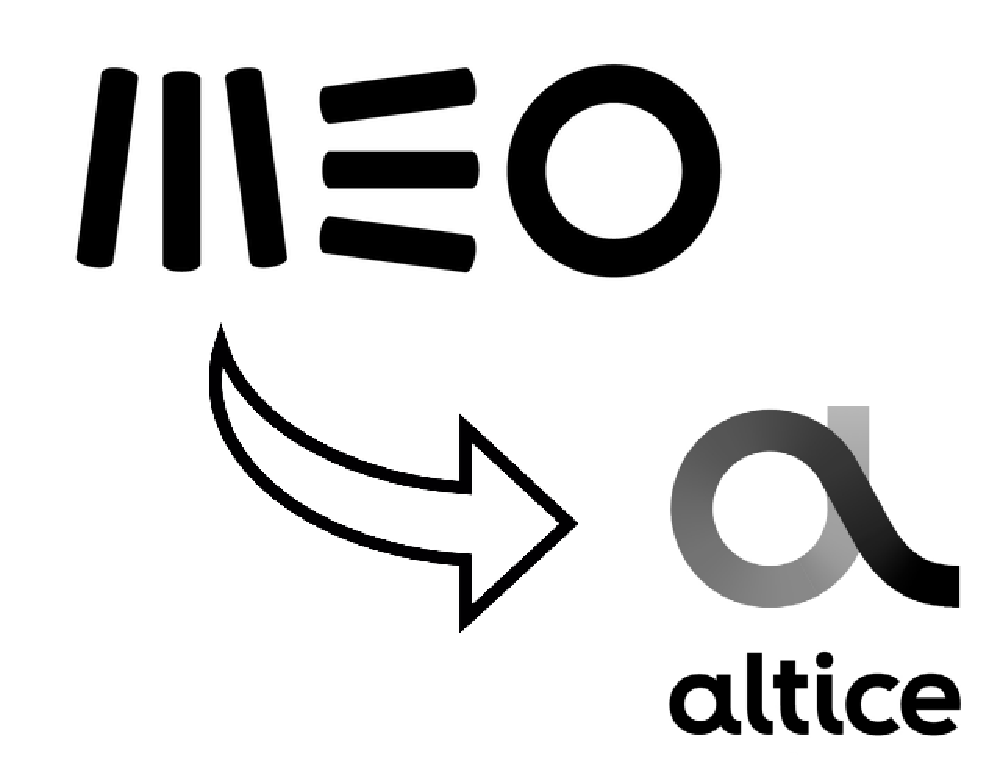
\includegraphics[width=4cm]{MEO-Altice.pdf} 
\begin{figure}[h]
\caption{Evolução da MEO em 2018 (editada)\href{https://pplware.sapo.pt/wp-content/uploads/2017/07/MEO-1-720x296.jpg}{[1]}\href{http://altice.net/sites/default/files/brand/altice_logo_pos_pr_rgb.jpg}{[2]}}
\end{figure}
\end{center}

\paragraph{Curiosidade:}

\paragraph{}A Meo encontra-se atualmente no 137º lugar da lista das marcas de telecomunicações mais valiosas do mundo, segundo a lista da \textit{Brand Finance}.

\chapter{Serviços}
\label{chap.serviços}

\section{Televisão}

\paragraph{}Uma das novidades da tecnologia \textit{IPTV} oferecida pela MEO é a possibilidade de as compras de canais poderem ser feitas diretamente nas casas dos clientes e através dos seus comandos, ao contrário dos serviços disponibilizados através de satélite e de cabo coaxial onde é necessário contactar a operadora para proceder à compra dos mesmos. Outra vantagem desta tecnologia \textit{IPTV} é o seu \textit{zapping}, ou seja, mudança de canal, considerado rápido, rondando os 200 milissegundos. Existe também a possibilidade de fazer um aluguer direto de filmes do Videoclube virtual onde estão presentes vários milhares de títulos, entre eles os mais recentes. A rede \textit{IPTV} ainda permite executar programas relacionados com os jogos na própria box e aceder a conteúdos da \textit{Internet} e a dezenas de aplicações interativas que englobam todos os gostos e conteúdos. Contem uma funcionalidade capaz de ter sempre disponível toda a programação dos canais, a chamada \textit{EPG}, e ativar ao mesmo tempo que se vê um canal escolhido pelo usuário, uma janela de visualização de outro canal sem que exista qualquer tipo de interrupção.

\section{\textit{Internet}}

\paragraph{}O serviço de acesso à \textit{Internet} por parte da MEO oferece uma grande variedade de larguras de banda larga, que depende obviamente do tipo de serviço escolhido por parte do cliente. Esta variedade é baseada nos dois tipos de rede existentes: rede de cobre \textit{ADSL2+} e rede de \textit{FTTH} (vulgarmente conhecida como Fibra Ótica). 

\paragraph{}Aprofundando os conhecimentos sobre o \textit{ADSL}, sabemos que para além do chamado \textit{ADSL} original, existe também o \textit{ADSL2} e o \textit{ADSL2+}, que oferecem taxas de \textit{download}, respetivamente, de 12 megabits e 24 megabits. O \textit{ADSL2} trabalha na mesma faixa de frequência do \textit{ADSL}, sendo esta desde os 26 kHz a 1100 kHz, enquanto que o \textit{ADSL2+} usa uma faixa dita de mais ampla, que vai desde os 26 kHz a 2200 kHz, o que permite dobrar a taxa de \textit{download}. A grande limitação é que, em ambos os casos, a taxa de \textit{upload} é mantida ficando em apenas 1 megabit. A largura de banda, pode ser reduzida quando o serviço de televisão se encontra ativo.

\begin{center}
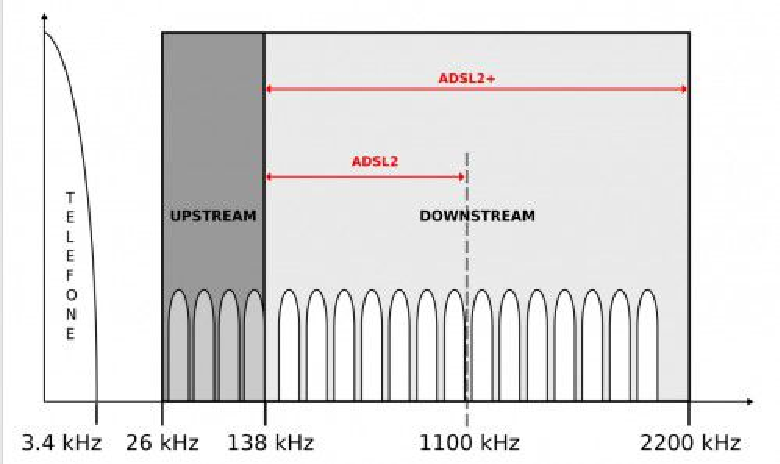
\includegraphics[width=9cm]{ADSL.pdf} 
\begin{figure}[h]
\caption{Gráfico comparativo entre ADSL, ADSL2, ADSL2+ \href{http://e.cdn-hardware.com.br/static/20140313/redes-adsl2re1.png.499x297.auto.jpg?CmsZoomEnable}{[3]}}
\end{figure}
\end{center}

\paragraph{}Na rede de fibra \textit{FTTH}, as larguras de banda larga, atingem um máximo de 1 Gbps em \textit{download} e 100 Mbps em \textit{upload}. Nesta rede o serviço não é afetado durante a utilização do serviço prestado de televisão.

\section{Telefone / Telemóvel}

\paragraph{}O serviço de telefone disponibiliza chamadas grátis e sem limites para todas as redes fixas nacionais e os seus custos são integrados pela assinatura do MEO.

\paragraph{}O serviço de telemóvel oferecido contem uma variedade de tarifários que se dividem em três categorias principais: pré-pagos, pós-pagos e os que são incluídos na fatura do serviço fixo (M40 e M50). O serviço de telemóvel é fornecido com recurso a uma cobertura de rede 2G, 3G e 4G.
\paragraph{}Os tarifários pré-pagos atualmente em vigor são: Top, Flex, Start, Moche e o MEO Kids.

\paragraph{}Os tarifários pós-pagos atualmente em vigor são: Unlimited S, Unlimited M, Unlimited L, Unlimited XL.

\newpage
 
\section{Apps MEO}

\paragraph{MEO Kanal:}

\paragraph{}O MEO Kanal oferece a possibilidade de criar um canal com as fotos e vídeos pessoais dos clientes, mantendo-o atualizado de forma fácil e de forma a que seja possível ver em todos os ecrãs. Os ficheiros (fotos e vídeos) guardados estarão sempre em segurança, podendo ser definido um \textit{PIN} pessoal. Existe a opção de tornar o canal público ou privado, consoante a decisão do usuário. Isto tudo é grátis para clientes MEO com TV, sem limites de armazenamento e com tráfego na rede móvel MEO incluído.

\paragraph{MEO Music:}

\paragraph{}É um serviço MEO de musica em \textit{streaming} que pode ser utilizado na TV, num PC e \textit{Macintosh} e também em terminais \textit{Android}, \textit{iOS} e \textit{Windows Phone}. Possui mais de 30 milhões de músicas e 1 milhão de videoclips. É gratuito para todos os clientes Moche, e para a maioria dos clientes MEO, porém qualquer pessoa pode experimentar o serviço durante 3 meses gratuitamente.

\paragraph{MEO Smart Home:}

\paragraph{}O MEO Smart Home disponibiliza ao cliente uma forma fácil de controlar e monitorizar remotamente a sua casa, informando-o da ocorrência de eventos relacionados com os vários detetores ao longo da casa. Esta informação é transmitida através de \textit{SMS}, email e notificações no seu telemóvel, PC ou tablet.

\paragraph{}Permite por exemplo:

\begin{itemize}
\item[•]A deteção de incidentes (intrusão, fumo, fugas de água);
\item[•]A deteção do consumo excessivo de energia;
\item[•]A Mediação de níveis de conforto de temperatura e humidade do ambiente;
\item[•]Gerir os destinatários de alertas, através da configuração de até 2 números de telemóvel e 2 endereços de email;
\item[•]Aceder em tempo real à(s) câmara(s) de vídeo MEO Smart Home, a partir do smartphone, computador ou tablet;
\item[•]Efetuar gravações de vídeo, a partir da(s) câmara(s) MEO Smart Home;
\item[•]Visualizar as gravações efetuadas com a(s) câmara(s) MEO Smart Home, por um período máximo de 30 dias a partir da data de gravação;
\item[•]Beneficiar de suporte técnico 24/24h através do 808 200 010, sempre que existirem problemas, ou dificuldades na utilização do serviço.
\end{itemize}

\chapter{Equipamento}
\label{chap.equipamento}

\paragraph{}Integrados nos serviços MEO residencial, os equipamentos disponibilizados, incluindo os comandos, vão variando em primeiro lugar na plataforma (\textit{ADSL}, fibra ou satélite) e em segundo no tarifário escolhido.

\paragraph{Rede satélite:}

\paragraph{}Com o MEO Satélite é possivel ter até duas MEOBoxes, podendo uma delas ter um gravador digital integrado, que permite ao utilizador gravar até um total de 300 horas. Os equipamentos disponiblizados nesta plantaforma são uma antena parabólica com um \textit{Low Noise Block (LNB)} e uma MEOBox que descodifica o sinal.
\paragraph{}A função da antena parabólica é apenas receber o sinal de televisão via satélite que por sua vez é descodificado por parte da MEOBox que o cliente possui em casa. Esta antena tem de estar virada para o satélite \textit{HISPASAT} (satélite responsável pelas telecomunicações por parte de Espanha e Portugal) e não pode ter objetos que impeçam o seu campo de ação.

\begin{center}
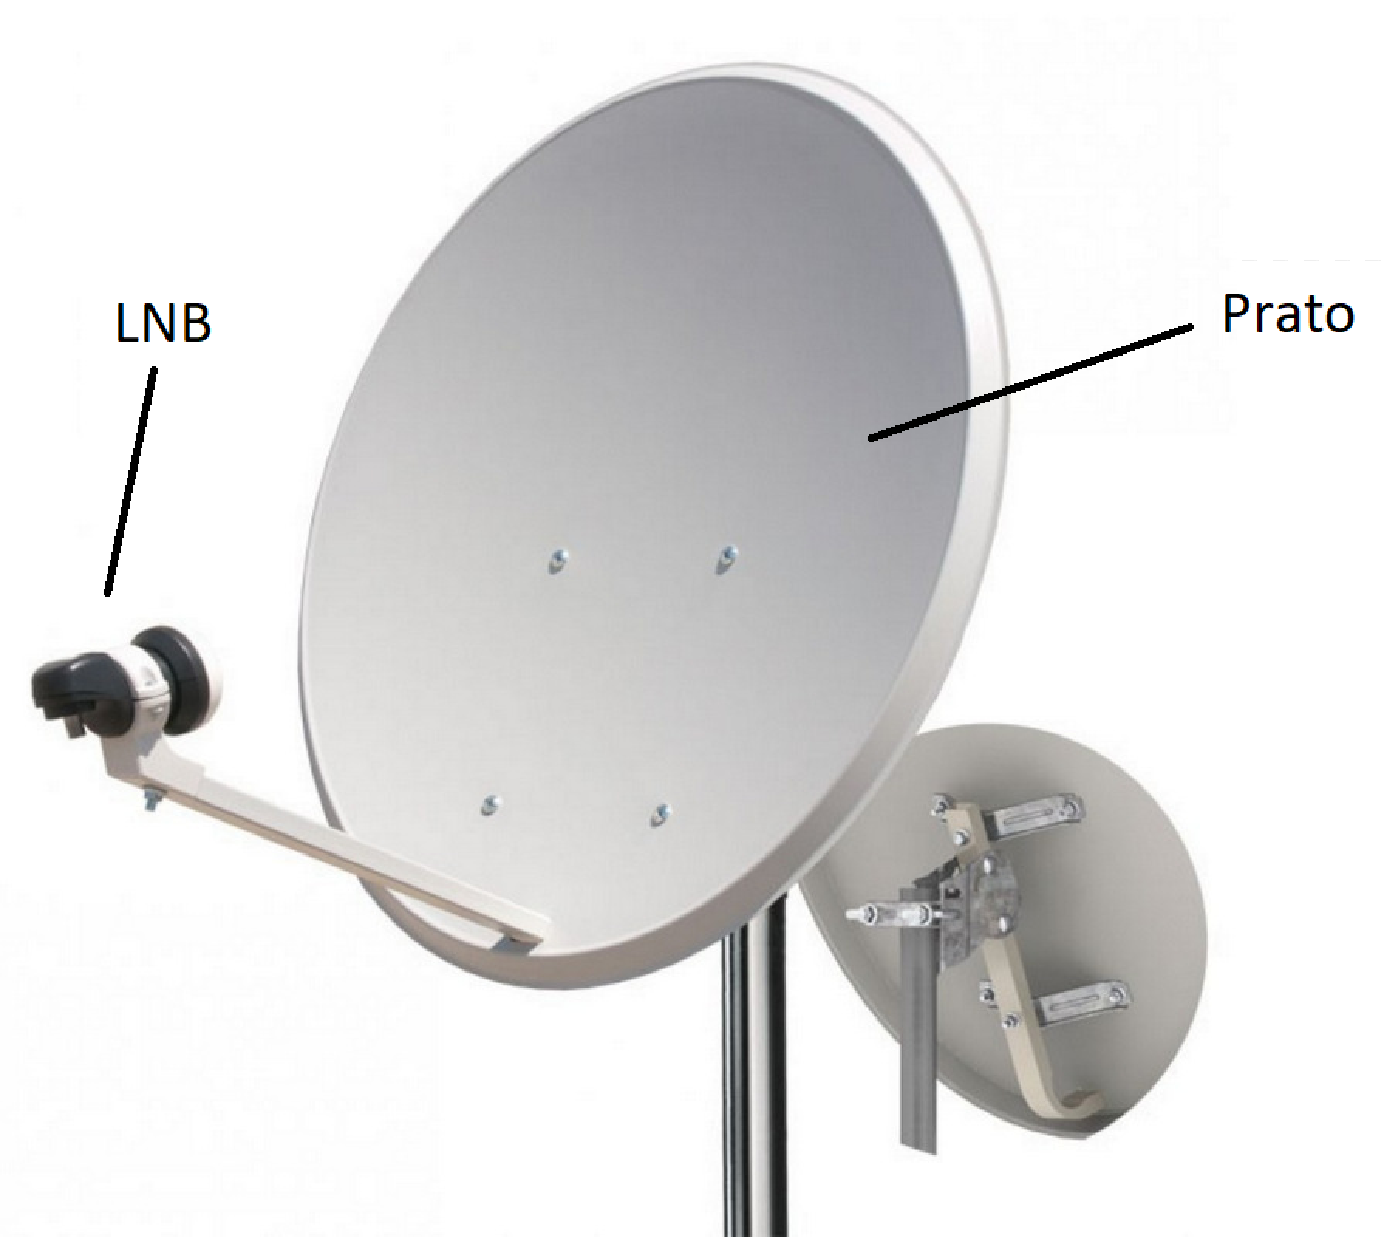
\includegraphics[width=47mm]{Parabolica.pdf} 
\begin{figure}[h]
\caption{Exemplo de uma parabólica (editada) \href{https://img.pccomponentes.com/articles/2/22673/kit-antena-parabolica-60cm-lnb-soporte-pared-1.jpg}{[4]}}
\end{figure}
\end{center}

\paragraph{}Por sua vez, o \textit{Low Noise Block (LNB)}, que é instalado na antena do MEO Satélite converte e amplifica a frequência recebida pela antena parabólica. Resumindo, o prato da antena recebe o sinal que é transmitido através do satélite \textit{HISPASAT}, e o \textit{LNB} amplifica-o e converte-o para ser descodificado pela MEOBox.

\paragraph{\textit{ADSL}:}

\paragraph{}Se o serviço for aravés da MEO \textit{ADSL}, o cliente tem a possibilidade de poder ter até duas MEOBoxes, porém, apenas a primeira MEOBox poderá conter um gravador digital que permite a gravação até 280 horas. Para a descodificação do sinal no caso do MEO por \textit{ADSL}, o serviço integra um conjunto de equipamentos a serem instalados no domicílio: um router com \textit{switch}, ligado à ficha telefónica através de um plug \textit{RJ}-14 para a descodificação e distribuição do sinal, com a possibilidade de ter de ser usado um \textit{splitter} (dependendo do router utilizado), e um aparelho descodificador para a Televisão, denominado MEOBox. 

\paragraph{}A MEOBox existe em vários modelos, sendo as mais utilizadas fabricadas pela Motorola e pela Scientific Atlanta, apresentando um processador, um disco rígido ou não, uma saída \textit{HDMI}, duas saídas \textit{SCART}, saída de som digital (ótico ou coaxial, dependendo do modelo da box instalada) e uma entrada para o cabo de \textit{Ethernet} que vem do router.

\paragraph{}Um \textit{Registered Jack (RJ)} é uma interface de rede de telecomunicações usada para ligar equipamentos de voz e dados a um serviço fornecido por uma operadora local. As tomadas registradas são nomeadas, primeiramente pelas letras \textit{RJ}, seguidas por dois dígitos que expressam o tipo. O plug \textit{RJ}-14, por exemplo, usa um conector modular 6P4C (6 pinos e 4 fios) e é utilizado para conexões telefónicas para serviços de duas linhas \href{https://pt.wikipedia.org/wiki/RJ_(conector)}{(link)}.

\begin{center}
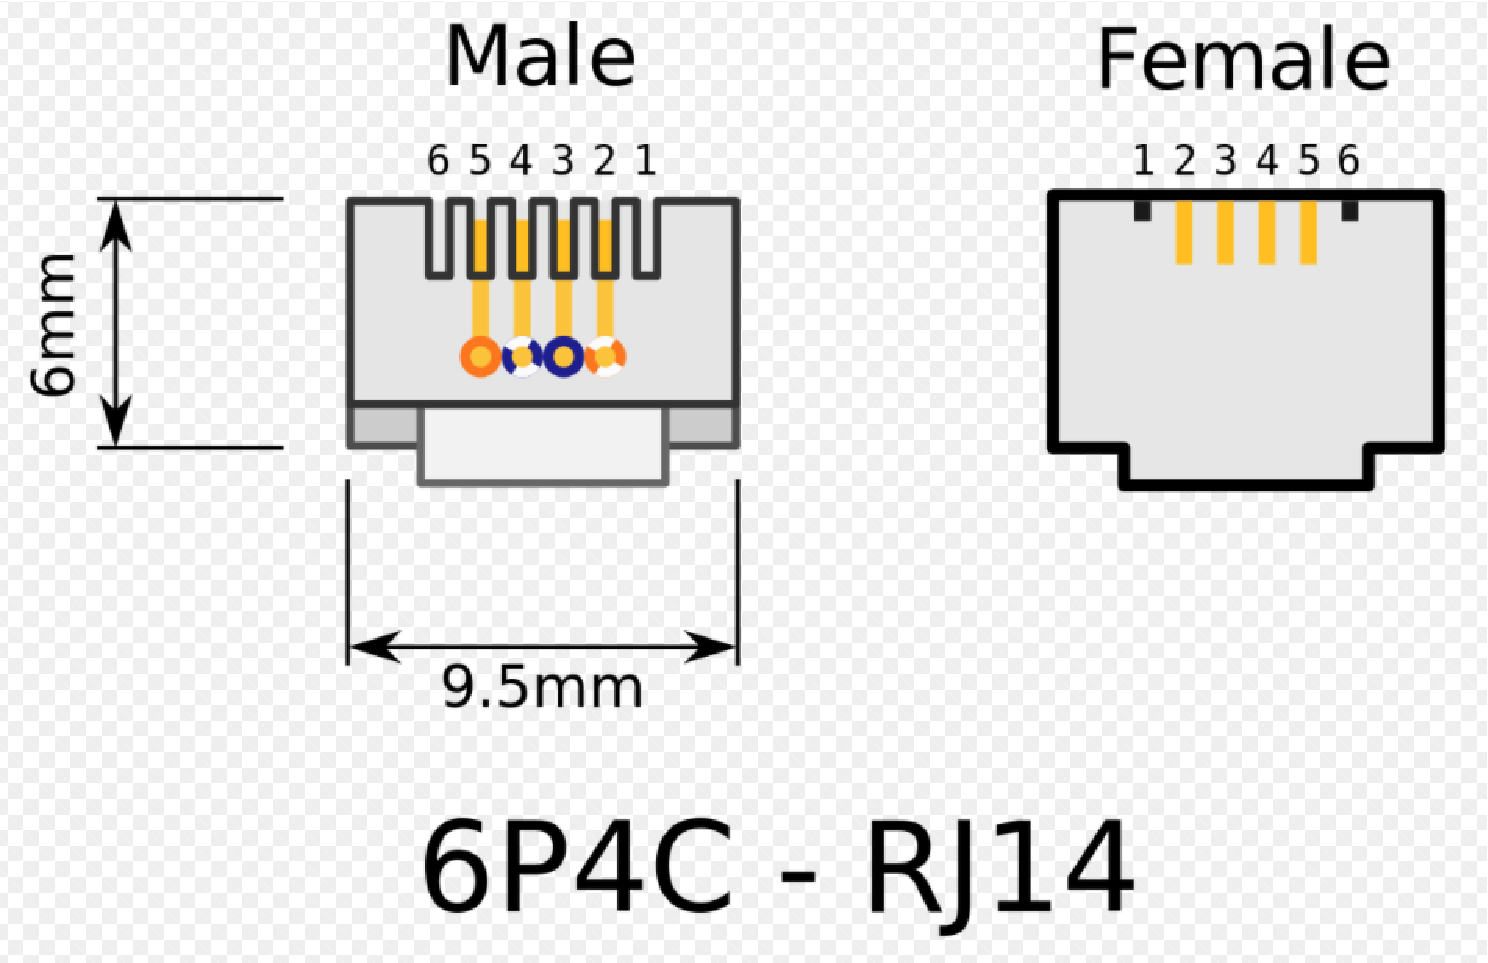
\includegraphics[width=6cm]{RJ14.pdf} 
\begin{figure}[h]
\caption{\textit{RJ}14 \href{https://upload.wikimedia.org/wikipedia/commons/c/c6/RJ14.svg}{[5]}}
\end{figure}
\end{center}

\newpage

\paragraph{}Os \textit{splitters} eram usados nos routers mais antigos para convergir os cabos da entrada telefónica e os da \textit{ADSL}, devido á existência de apenas uma entrada no router. Nos routers de hoje em dia já não é preciso um \textit{splitter}, pois já possuem duas entradas\href{https://www.ispblog.com.br/2016/10/31/splitter-entenda-o-que-e-e-os-seus-modelos/}{(link)}.

\begin{center}
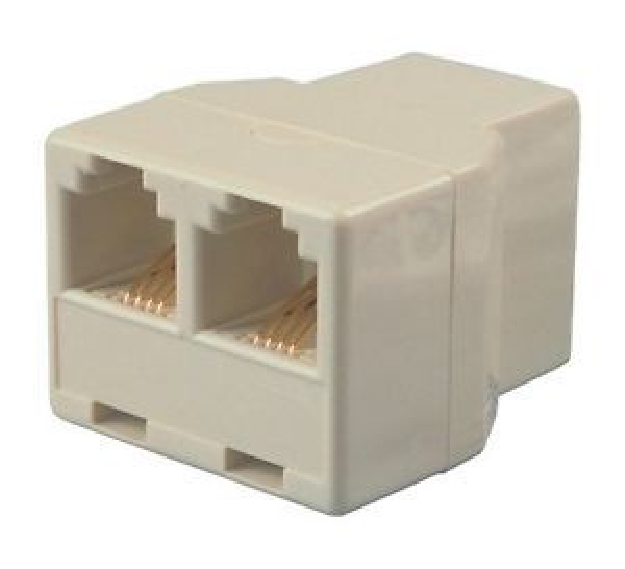
\includegraphics[width=3cm]{Splitter_RJ14.pdf} 
\begin{figure}[h]
\caption{Splitter \textit{RJ}14\href{https://i.ebayimg.com/images/g/CtUAAOSwaNBUg8Aj/s-l300.jpg}{[6]}}
\end{figure}
\end{center}

\paragraph{Fibra Ótica:}

\paragraph{}O serviço MEO Fibra permite instalar até 3 MEOBoxes em casa dos clientes. Se o cliente possuir em casa uma rede de tomadas de televisão (rede coaxial), é possível ter acesso a canais do MEO nas restantes televisões da casa. Porém se essas televisões não tiverem uma MEOBox, não haverá acesso aos serviços interativos disponiblizados pela MEO.

\paragraph{}No que toca a equipamentos no caso do MEO por fibra ótica, é acresentado um equipamento adicional que se chama \textit{ONT- Optical Network Terminal}, que descodifica o sinal da fibra ótica enviado até a casa dos cliente, e envia para o router. Para além de injetar sinal de televisão na rede coaxial, tornando-se assim num serviço de \textit{IPTV}, é possível deixar a necessidade de ter uma box por cada televisão de lado.

\begin{center}
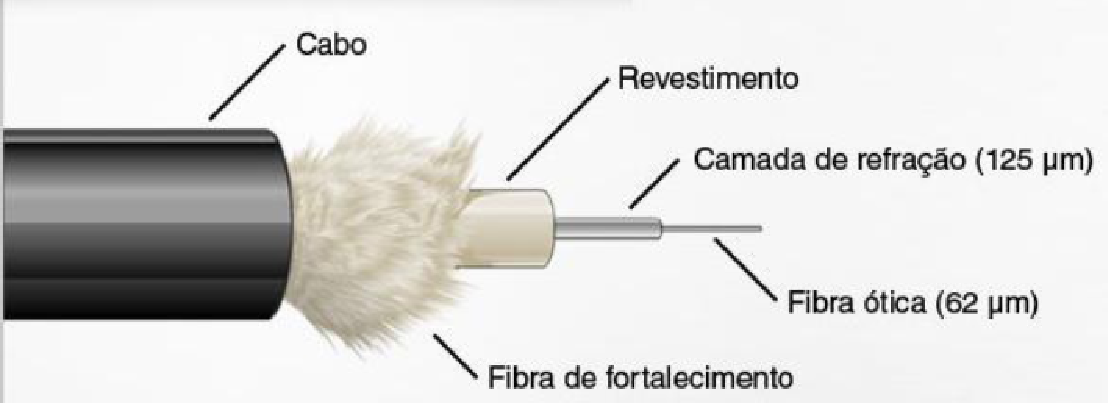
\includegraphics[width=8cm]{fibra_otica.pdf} 
\begin{figure}[h]
\caption{Constituição da fibra ótica\href{http://www.projetoderedes.com.br/artigos/imagens/Image9.png}{[7]}}
\end{figure}
\end{center}

\newpage

\paragraph{Resumo das ligações de todos os tipos da MEO:}

\begin{center}
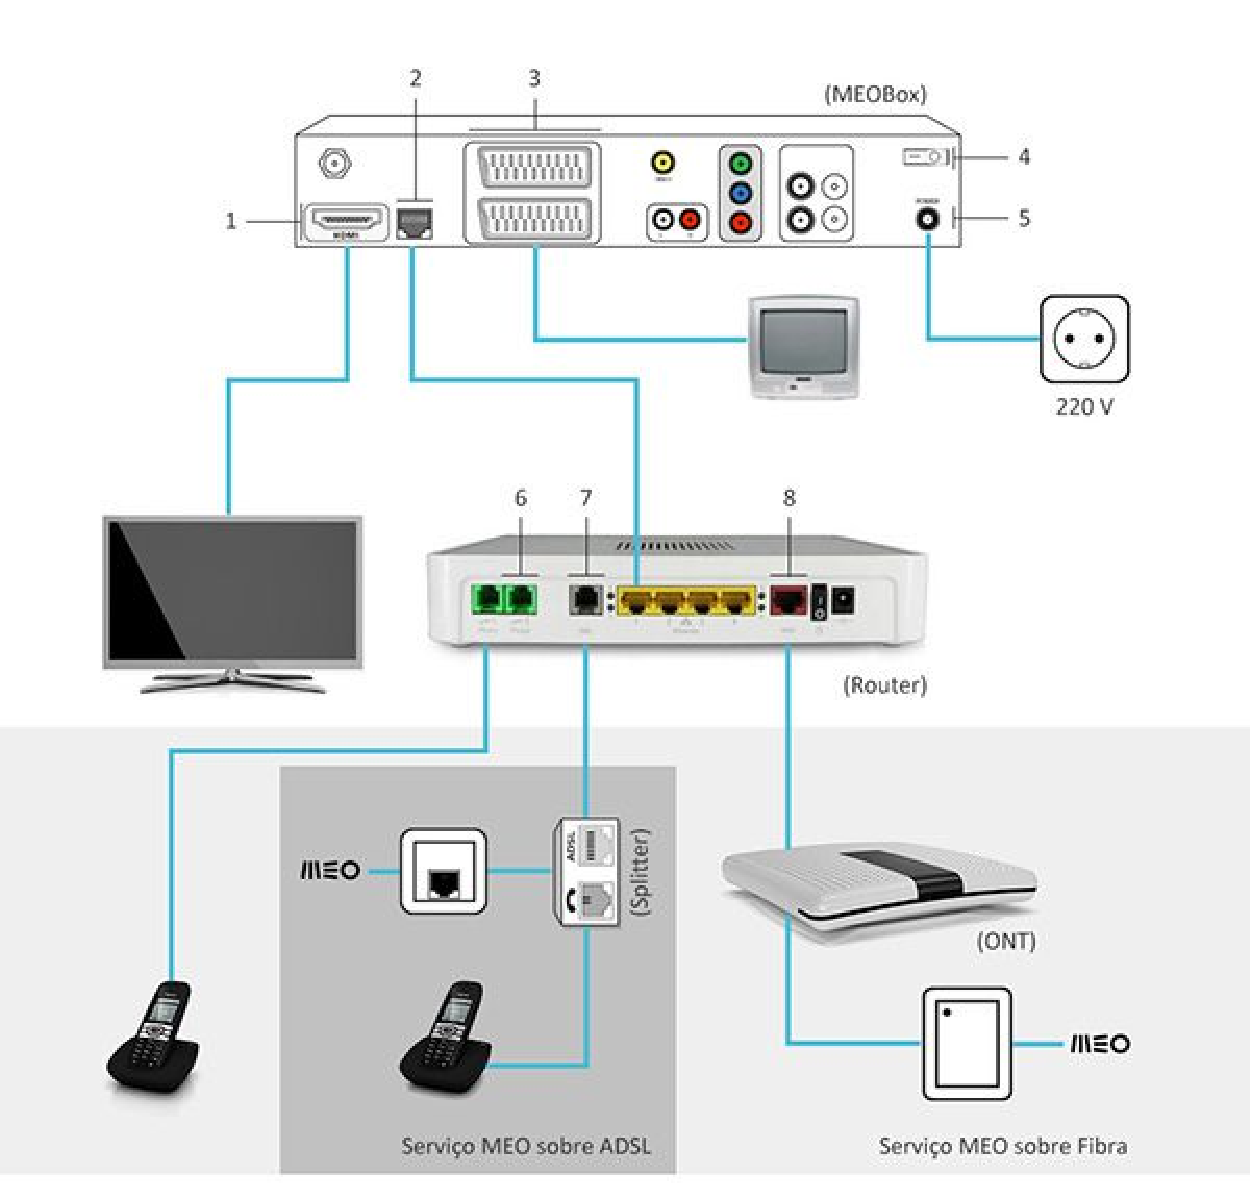
\includegraphics[width=10cm]{Todas_as_ligacoes_(MEO).pdf} 
\begin{figure}[h]
\caption{Todas as ligações \href{https://conteudos.meo.pt/meo/UCMImages/CustomerCare/2013/ESQUEMA-detalhado-todas-ligacoessemlegenda.jpg}{[8]}}
\end{figure}
\end{center}

\paragraph{Exemplo de uma MEOBox (Motorola VIP1200 Serie):}

\paragraph{} A Motorola VIP1200 Series primária, que efectua a ligação à televisão principal, pode conter um gravador de vídeo digital (\textit{DVR}) permitindo assim a funcionalidade de gravação automática. Este \textit{DVR} pode gravar programas com definição normal ou em alta definição num disco rígido. Também permite fazer uma pausa e regressar atrás em caso de programação ao vivo, mas esta funcionalidade pode ser limitada em alguns canais, dependendo do suportado por este. Uma Motorola VIP1200 secundária é usada para as televisões adicionais que existem no resto da casa. Normalmente a Motorola primária VIP1208/1216/1232 é maior do que a Motorola secundária VIP1200, visto que a primeira possuiu um espaço adicional para alojar o disco rígido para o \textit{DVR} \href{https://conteudos.meo.pt/meo/Documentos/Manuais/Box/MEO-Fibra-ADSL/Manual-Instalacao-Motorola.pdf}{(link)} .

\newpage

\paragraph{}Os números de modelos da Box Motorola VIP são:

\begin{itemize}
\item[•]VIP1200 não possui um \textit{DVR};
\item[•]VIP1208 com um disco rígido de 80 GByte;
\item[•]VIP1216 com um disco rígido de 160 GByte;
\item[•]VIP1232 com um disco rígido de 320 GByte.
\end{itemize}

\begin{center}
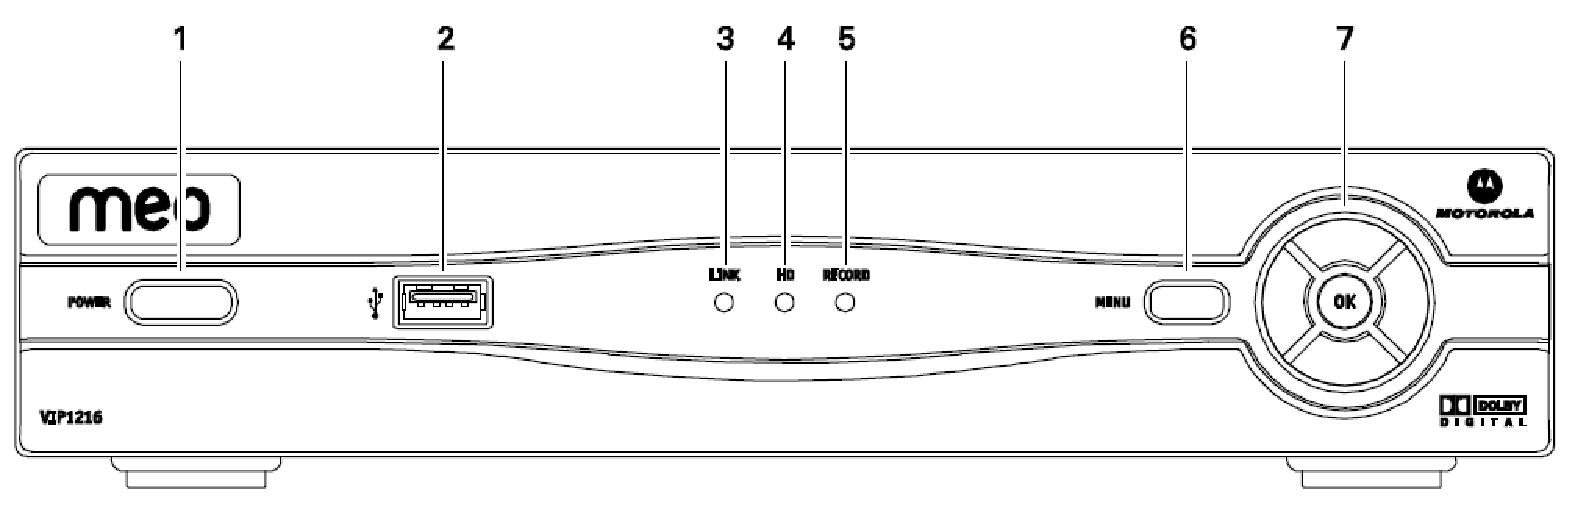
\includegraphics[width=12cm]{Motorola_VIP1200_Serie-Painel_Frontal.pdf} 
\begin{figure}[h]
\caption{Motorola VIP1200 Serie-Painel Frontal\href{https://conteudos.meo.pt/meo/Documentos/Manuais/Box/MEO-Fibra-ADSL/Manual-Instalacao-Motorola.pdf}{[9]}}
\end{figure}
\end{center}

\begin{center}
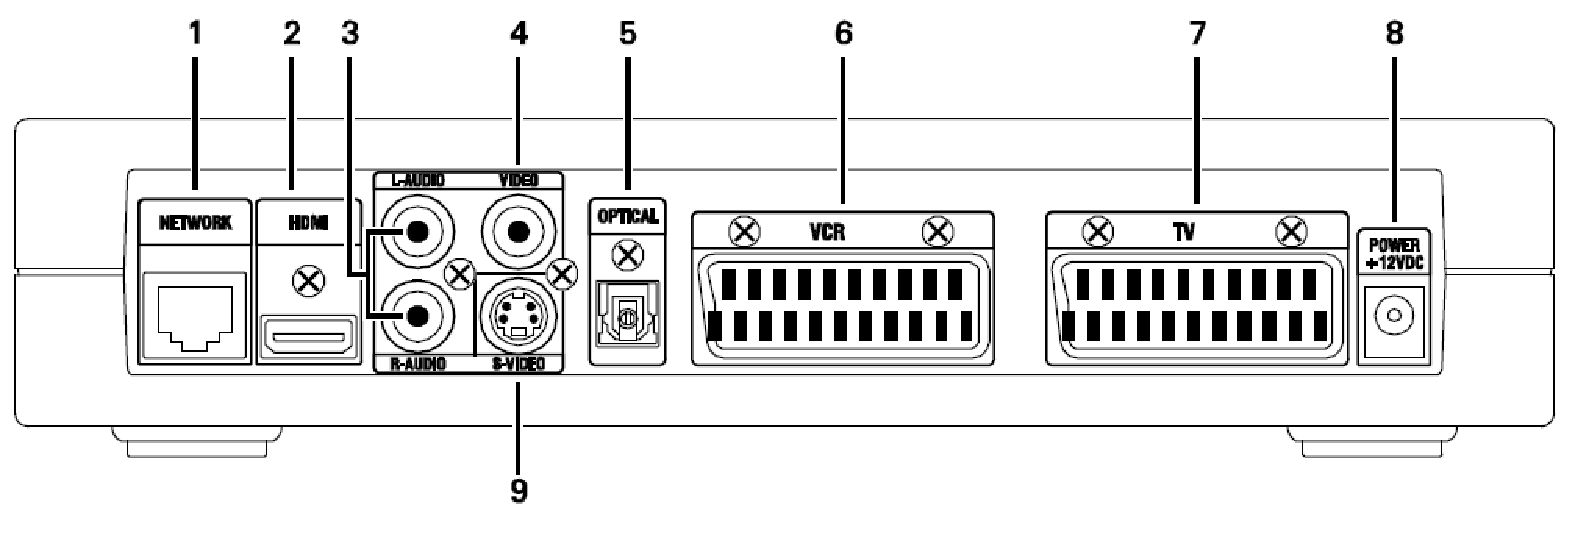
\includegraphics[width=12cm]{Motorola_VIP1200_Serie-Painel_Traseiro.pdf} 
\begin{figure}[h]
\caption{Motorola VIP1200 Serie-Painel Traseiro\href{https://conteudos.meo.pt/meo/Documentos/Manuais/Box/MEO-Fibra-ADSL/Manual-Instalacao-Motorola.pdf}{[10]}}
\end{figure}
\end{center}

\chapter{Cobertura e Tecnologias}
\label{chap.coberturaEtecnologias}

Como já referimos acima, a empresa MEO disponibiliza 4 tipos de serviços: tv, net, voz e rede móvel. Os serviços de Televisão, \textit{Internet} e Telefone Fixo são distribuídos para as casas dos consumidores através de uma das três tecnologias que a MEO disponibiliza, pode ser então por fibra ótica, \textit{ADSL} ou satélite.
 
	As duas primeiras tecnologias têm um funcionamento que se baseia num \textit{IPTV (Internet Protocol Television)}, um método de transmissão de sinais televisivos. Neste, o conteúdo é enviado em \textit{streaming} a partir da \textit{internet}, porém, usando uma infraestrutura dedicada, paralela á “\textit{internet} comum” para poder garantir a qualidade e velocidade do serviço.

	A última tem um funcionamento que se baseia num \textit{DTH (Direct To Home)}, é também um método de transmissão de sinais televisíveis, mas por satélite. Esta tecnologia é também usada pela \textit{TDT (Televisão Digital Terrestre)}.

\paragraph{}
	Para poder comparar as características de cada uma das tecnologias, teremos em conta o pacote M4O que contém os 4 serviços: Televisão, \textit{Internet}, Telefone Fixo e Telemóvel. Isto porque este pacote está presente em todas as tecnologias que a MEO disponibiliza. O pacote tem um preço de 56,99\euro{} independentemente da tecnologia escolhida.
 
	No que diz respeito á fibra ótica, a MEO disponibiliza 200 canais de televisão e \textit{Internet} com velocidades de 100 Mbps de \textit{download} e \textit{upload}. Esta tecnologia não está presente em todo o país, pelo que se encontra apenas nas grandes cidades. 

	Em alternativa temos \textit{ADSL} que disponibiliza também 200 canais de televisão, mas em contrapartida a velocidade máxima da Internet é de apenas 24 Mbps. A \textit{ADSL} é uma tecnologia de comunicação de dados que permite a transmissão de dados através da linha de telefone. Esta tem algumas limitações visto que é bastante comum a queda de velocidade de \textit{Internet} aquando da utilização do serviço de televisão. Esta é bastante mais disponível pelo país do que a primeira, mas tem as suas limitações. 

	Por ultimo temos satélite que disponibiliza 90 canais de televisão e 40 Mbps de \textit{Internet}. Esta tecnologia tem as suas limitações em comparação ás outras duas apresentadas, mas em contrapartida é a única tecnologia que cobre a totalidade do território nacional.

	Cada uma destas tecnologias tem as suas particularidades e são aplicadas consoante disponibilidade e necessidade dos consumidores \href{https://www.meo.pt/pacotes}{(link)}.

	No que diz respeito aos serviços móveis, a MEO disponibiliza as redes 3G e 4G. Segundo a MEO, os valores estimados da velocidade máxima de \textit{Internet} para a rede 3G é de 16 Mbps de \textit{download} e 5 Mbps de \textit{upload}. Para a rede 4G a velocidade máxima (estimada) de \textit{download} é de 80Mbps e 40 Mbps de \textit{upload} \href{https://conteudos.meo.pt/meo/Documentos/Condicoes-Oferta-Servicos/Mod-C1001276.pdf}{(link)}. Em termos de cobertura do sinal, como podemos visualizar na (Figura \ref{Figura 11}) a rede 4G está principalmente presente no litoral, mas podemos visualizar que os distritos de Beja e Évora também têm uma boa cobertura. A rede 3G, por outro lado está presente em grande parte do país deixando poucas zonas com cobertura apenas 2G.

	A MEO oferece, portanto, 4 tipos de serviços, cada um com as suas particularidades e serão usados consoante a necessidade de cada um dos consumidores que aderirem aos serviços da MEO.
	
	
\begin{center}
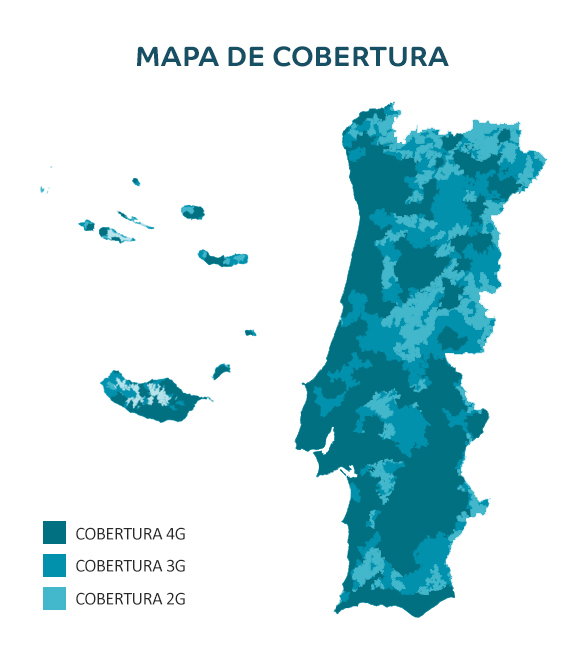
\includegraphics[width=5cm]{fig8.jpeg} 
\begin{figure}[h]
\caption{Mapa de Cobertura \href{https://kptuy52666.i.lithium.com/t5/image/serverpage/image-id/169i59E9D89E18800D60/image-size/original?v=mpbl-1&px=-1}{[11]}}
\label{Figura 11}
\end{figure}
\end{center}


\chapter{Concorrência}
\label{chap.concorrência}


A MEO é uma empresa de Serviços de Comunicação e Multimédia com uma presença no mercado bastante forte desde já uns anos, mas não está sozinha no território nacional. As principais empresas concorrentes são a NOS, a Vodafone e a Nowo \textit{(Grupo APAX)}. 

\paragraph{}
	Embora a MEO tenha sido líder no mercado, os números divulgados pela \textbf{ANACOM} \href{https://www.anacom.pt/streaming/PacotesServicos1T17_final.pdf?contentId=1410761&field=ATTACHED_FILE}{(link)} revelam que no primeiro trimestre de 2017, a NOS consegui ultrapassar o número total de subscritores de pacotes de serviços de comunicações da MEO. 
	
	Em termos de percentagens, a MEO registou uma quota de mercado de cerca de 39,2\%, a NOS consegui obter 39,4\%, a Vodafone obteve 16,4\% e o \textit{Grupo APAX}, onde a Nowo se insere registou 5\%. A MEO lidera nas modalidades 2P (televisão e \textit{internet} ou telefone e \textit{internet}) e 5P (contém também a banda larga móvel) enquanto que a NOS liderava nas modalidades 3P e 4P (televisão, \textit{internet}, telefone e rede móvel).
	 
	Embora a NOS tenha mais clientes, a MEO continua a bater nas receitas, dados divulgados pela \textit{ANACOM} \href{https://www.anacom.pt/streaming/PacotesServicos1T17_final.pdf?contentId=1410761&field=ATTACHED_FILE}{(link)} revelam que a MEO tem cerca de 41,8\% da quota do mercado em termos de receitas, enquanto que a NOS tem apenas 39,9\%. Atrás da NOS, temos a Vodafone com 14,2\% e o \textit{(Grupo APAX)} com 4\%.

\paragraph{}	
	No que toca a serviços e tecnologias prestadas por cada uma das entidades, a MEO lidera no mercado.
	
	A MEO oferece os 4 serviços: Televisão, \textit{Internet}, Telefone Fixo e Rede Móvel. No que toca a televisão, \textit{internet} e telefone fixo, a empresa disponibiliza, como já referido acima, as seguintes tecnologias: fibra ótica, \textit{ADSL} e satélite, sendo assim a única no país a prestar as 4 tecnologias.
	
	A NOS oferece também os 4 serviços, mas não possui tantas tecnologias quanto a MEO, em contrapartida oferece simplesmente satélite e fibra ótica, desta maneira não podendo chegar a tanto público.
	
	 A Vodafone oferece também 4 serviços, mas possui apenas as opções satélite e fibra ótica. Desta maneira poderá não chegar a todo o país visto que em zonas que não tenha linha telefónica nem fibra ótica, o serviço não poderá ser prestado.
	 
	Por último a Nowo \textit{(Grupo APAX)} oferece também os 4 serviços, mas tem apenas disponível a tecnologia fibra ótica o que limita bastante as zonas de prestações de serviços. Por esta mesma razão que a quota no mercado seja tão baixa. Limita a sua prestação de serviços a grandes cidades onde a fibra ótica está presente. 
	
\paragraph{}
	A MEO é, portanto, a marca que melhor está colocada no mercado em termos de receitas e em termos de tipos de tecnologias que presta aos seus clientes.
	

\chapter{Altice}
\label{chap.altice}

Como já referimos acima a MEO é uma marca criada pela \textit{PT (Portugal Telecom)}, marca essa que apareceu em 2007 através do lançamento do serviço \textit{triple play} da \textit{Portugal Telecom}.

	A \textit{PT (Portugal Telecom)} é detentora de marcas como a MEO, que já foi referida; a \textit{PT} Empresas, que dispõe de soluções tecnológicas e de telecomunicações especialmente pensadas para pequenas e médias empresas, bem como para grandes empresas; e a SAPO (Servidor de Apontadores Portugueses Online), um portal português fornecedor de conteúdos digitais fundada em 1995 como um motor de pesquisa. 

\paragraph{}
	A 2 de Junho de 2015, a Altice (uma multinacional francesa de telecomunicações, conteúdos, media, entretenimento e publicidade) comprou a \textit{Portugal Telecom} por 5.8 mil milhões de euros. Como a MEO era uma marca que pertencia a \textit{PT}, passou assim a ser propriedade da Altice. 
	
	A 23 de Maio de 2017, foi anunciado que a marca MEO, assim como a marca \textit{Portugal Telecom}, irão desaparecer até ao segundo trimestre de 2018, passando ambas as marcas a designar-se Altice. Isto porque tem um objetivo de criar uma marca única para todos os países onde a Altice está presente. 
	
	No âmbito da criação da marca única, a Altice já tem mostrado que está empenhada em Portugal. A 17 de Outubro de 2017, a MEO Arena, que era propriedade da \textit{PT} passou a designar-se Altice Arena. No inicio de Novembro de 2017, a marca alterou o nome da rede MEO para Altice MEO, alteração que pode ser visualizada na parte superior do ecrã do telemóvel onde o nome da rede é mostrado.
	
\paragraph{}
	Podemos então apercebermo-nos que a marca MEO irá então desaparecer em favor da marca Altice, que passará a ser detentora de todas as conquistas que a marca MEO consegui ao longo dos anos.

\newpage

\chapter*{Glossário}

\paragraph{IPTV} Internet Protocol Television
\paragraph{EPG} Electronic Programming Guide
\paragraph{ADSL} Assymetrical Digital Subscriber Line
\paragraph{FTTH} Fiber to the Home
\paragraph{PIN} Personal Identification Number
\paragraph{ANACOM} Autoridade Nacional de Comunicações
\paragraph{SMS} Short Message Service
\paragraph{LNB} Low-noise block
\paragraph{HDMI} High-Definition Multimedia Interface 
\paragraph{SCART} Syndicat des Constructeurs d'Appareils Radiorécepteurs et Téléviseurs
\paragraph{RJ} Registered Jack
\paragraph{ONT} Optical Network Terminal
\paragraph{DVR} Digital Video Recorder
\paragraph{DTH} Direct to Home
\paragraph{PT} Portugal Telecom

\chapter*{Outros Links}

\begin{itemize}

\item[•] Dinheiro Vivo. Disponível em: \url{https://www.dinheirovivo.pt/empresas/as-voltas-que-a-meo-deu/}. Acesso em: 11 Novembro 2017.
\item[•] Hardware.com.br. Disponivel em: \url{http://www.hardware.com.br/livros/redes/adsl2-adsl2-adsl2-vdsl2.html}. Acesso em: 15 Novembro 2017.
\item[•] Motorola Mobility, Inc.(2011).A sua Set-Top Box IP TV Motorola VIP1200 Series. Set-Top Box IP TV Motorola VIP1200 Series Manual de Instalação.p.1,2,3.
\item[•] Meo. Disponível em: \url{https://www.meo.pt}. Acesso em: 11 Novembro 2017.
\item[•] Adslfibra. Disponível em: \url{https://adslfibra.pt/operadores-telecomunicacoes}. Acesso em: 11 Novembro 2017.
\item[•] Wikipédia. Disponível em: \url{https://pt.wikipedia.org/wiki/Meo}. Acesso em: 11 Novembro 2017.
\item[•] Wikipédia. Disponível em: \url{https://pt.wikipedia.org/wiki/Portugal_Telecom}. Acesso em: 11 Novembro 2017.
\item[•] Wikipédia. Disponível em: \url{https://pt.wikipedia.org/wiki/DTH}. Acesso em: 11 Novembro 2017.
\item[•] Wikipédia. Disponível em: \url{https://pt.wikipedia.org/wiki/IPTV}. Acesso em: 11 Novembro 2017.
\item[•] ECO. Disponível em: \url{https://eco.pt/2017/06/06/nos-ja-tem-mais-clientes-que-a-meo/}. Acesso em: 12 Novembro 2017.
\item[•] ECO. Disponível em: \url{https://eco.pt/2017/11/08/o-fim-da-marca-meo-esta-cada-vez-mais-proximo/}. Acesso em: 12 Novembro 2017.
\item[•] PT Portugal. Disponível em: \url{https://www.telecom.pt/pt-pt/a-pt/Paginas/marcas-pt.aspx}. Acesso em: 12 Novembro 2017.


\end{itemize}

\end{document}
